\documentclass[tikz,border=8pt]{standalone}

\usepackage[T1]{fontenc}
\usepackage{amsmath,amssymb}
\usepackage{xcolor}
\usepackage{helvet}
\renewcommand{\familydefault}{\sfdefault}
\usepackage{mathastext}
\usepackage{tikz}
\hyphenpenalty=10000 \exhyphenpenalty=10000 \tolerance=9999 \emergencystretch=3em
\usetikzlibrary{arrows.meta,calc,shadows}

\definecolor{ink}{RGB}{26,34,44}
\definecolor{muted}{RGB}{97,108,122}
\definecolor{hair}{RGB}{214,220,228}
\definecolor{navy}{RGB}{31,78,121}
\definecolor{navysoft}{RGB}{238,244,250}
\definecolor{amber}{RGB}{184,106,27}
\definecolor{ambersoft}{RGB}{253,245,234}
\definecolor{green}{RGB}{42,117,91}
\definecolor{greensoft}{RGB}{237,247,243}
\definecolor{red}{RGB}{150,40,40}
\definecolor{redsoft}{RGB}{250,236,236}

\newcommand{\fsTitle}{\fontsize{9.4}{11}\selectfont\bfseries}
\newcommand{\fsSub}{\fontsize{7.5}{9}\selectfont}
\newcommand{\fsCardT}{\fontsize{8.4}{10}\selectfont\bfseries}
\newcommand{\fsCardS}{\fontsize{7.5}{9}\selectfont}
\newcommand{\fsPill}{\fontsize{6.8}{8}\selectfont\bfseries}
\newcommand{\fsNote}{\fontsize{7.6}{9.4}\selectfont}
\newcommand{\fsTiny}{\fontsize{7.2}{8.2}\selectfont}

% boundary card: num, title, subtitle, accent, soft, note, half-width, full-width
\newcommand{\bchrome}[8]{%
	\node[rectangle, rounded corners=5pt, fill=white, draw=hair, line width=0.7pt,
	minimum width=#8mm, minimum height=80mm, inner sep=0pt,
	drop shadow={shadow xshift=0.7pt, shadow yshift=-1pt, opacity=0.09, fill=black}]
	at (0,0) {};
	\begin{scope}
		\clip[rounded corners=5pt] (-#7,-40) rectangle (#7,40);
		\shade[left color=#4, right color=#4!35] (-#7,38.9) rectangle (#7,40);
	\end{scope}
	\draw[hair, rounded corners=5pt, line width=0.7pt] (-#7,-40) rectangle (#7,40);
	\node[rounded corners=2.5pt, fill=ink, text=white, minimum width=7.5mm,
	minimum height=5mm, inner sep=0pt, font=\fontsize{6.8}{8}\selectfont\bfseries]
	at (-#7+8.25,34) {#1};
	\node[anchor=west, text=ink, font=\fsTitle] at (-#7+13.5,34) {#2};
	\pgfmathsetmacro{\subw}{2*#7-9}
	\node[anchor=north west, text=muted, text width=\subw mm, align=left, font=\fsSub]
	at (-#7+4.5,30.2) {#3};
	\draw[hair, line width=0.6pt] (-#7+4.5,23.2) -- (#7-4.5,23.2);
	\fill[#5, rounded corners=3.5pt] (-#7+4.5,-35) rectangle (#7-4.5,-22.4);
	\draw[#4, line width=1.5pt, line cap=round] (-#7+6.4,-24.4) -- (-#7+6.4,-33);
	\pgfmathsetmacro{\notew}{2*#7-17}
	\node[anchor=west, text=ink, text width=\notew mm, align=left, font=\fsNote]
	at (-#7+8.8,-28.7) {#6};
}

\newcommand{\pill}[5]{%
	\node[anchor=#4, rounded corners=2.2pt, fill=#1!11, text=#1!85!black,
	inner xsep=3pt, inner ysep=1.5pt, font=\fsPill] at (#2,#3) {#5};}

% finding row: x, y, width, accent, soft, title, subtitle, pill (may be empty)
\newcommand{\anode}[8]{%
	\draw[#4!70!black, fill=#5, line width=0.8pt, rounded corners=3.5pt]
	(#1-#3/2,#2-5) rectangle (#1+#3/2,#2+5);
	\draw[#4, line width=1.5pt, line cap=round] (#1-#3/2+2.1,#2-3.3) -- (#1-#3/2+2.1,#2+3.3);
	\node[anchor=west, text=ink, font=\fsCardT] at (#1-#3/2+4.8,#2+1.9) {#6};
	\node[anchor=west, text=muted, font=\fsCardS] at (#1-#3/2+4.8,#2-2.1) {#7};
	\ifx&#8&\else\pill{#4}{#1+#3/2-2.2}{#2+5}{east}{#8}\fi}

\tikzset{flow/.style={->, navy!75, line width=1.1pt, rounded corners=2.5pt},
	elab/.style={text=muted, font=\fsTiny\bfseries, inner sep=1pt}}

\begin{document}
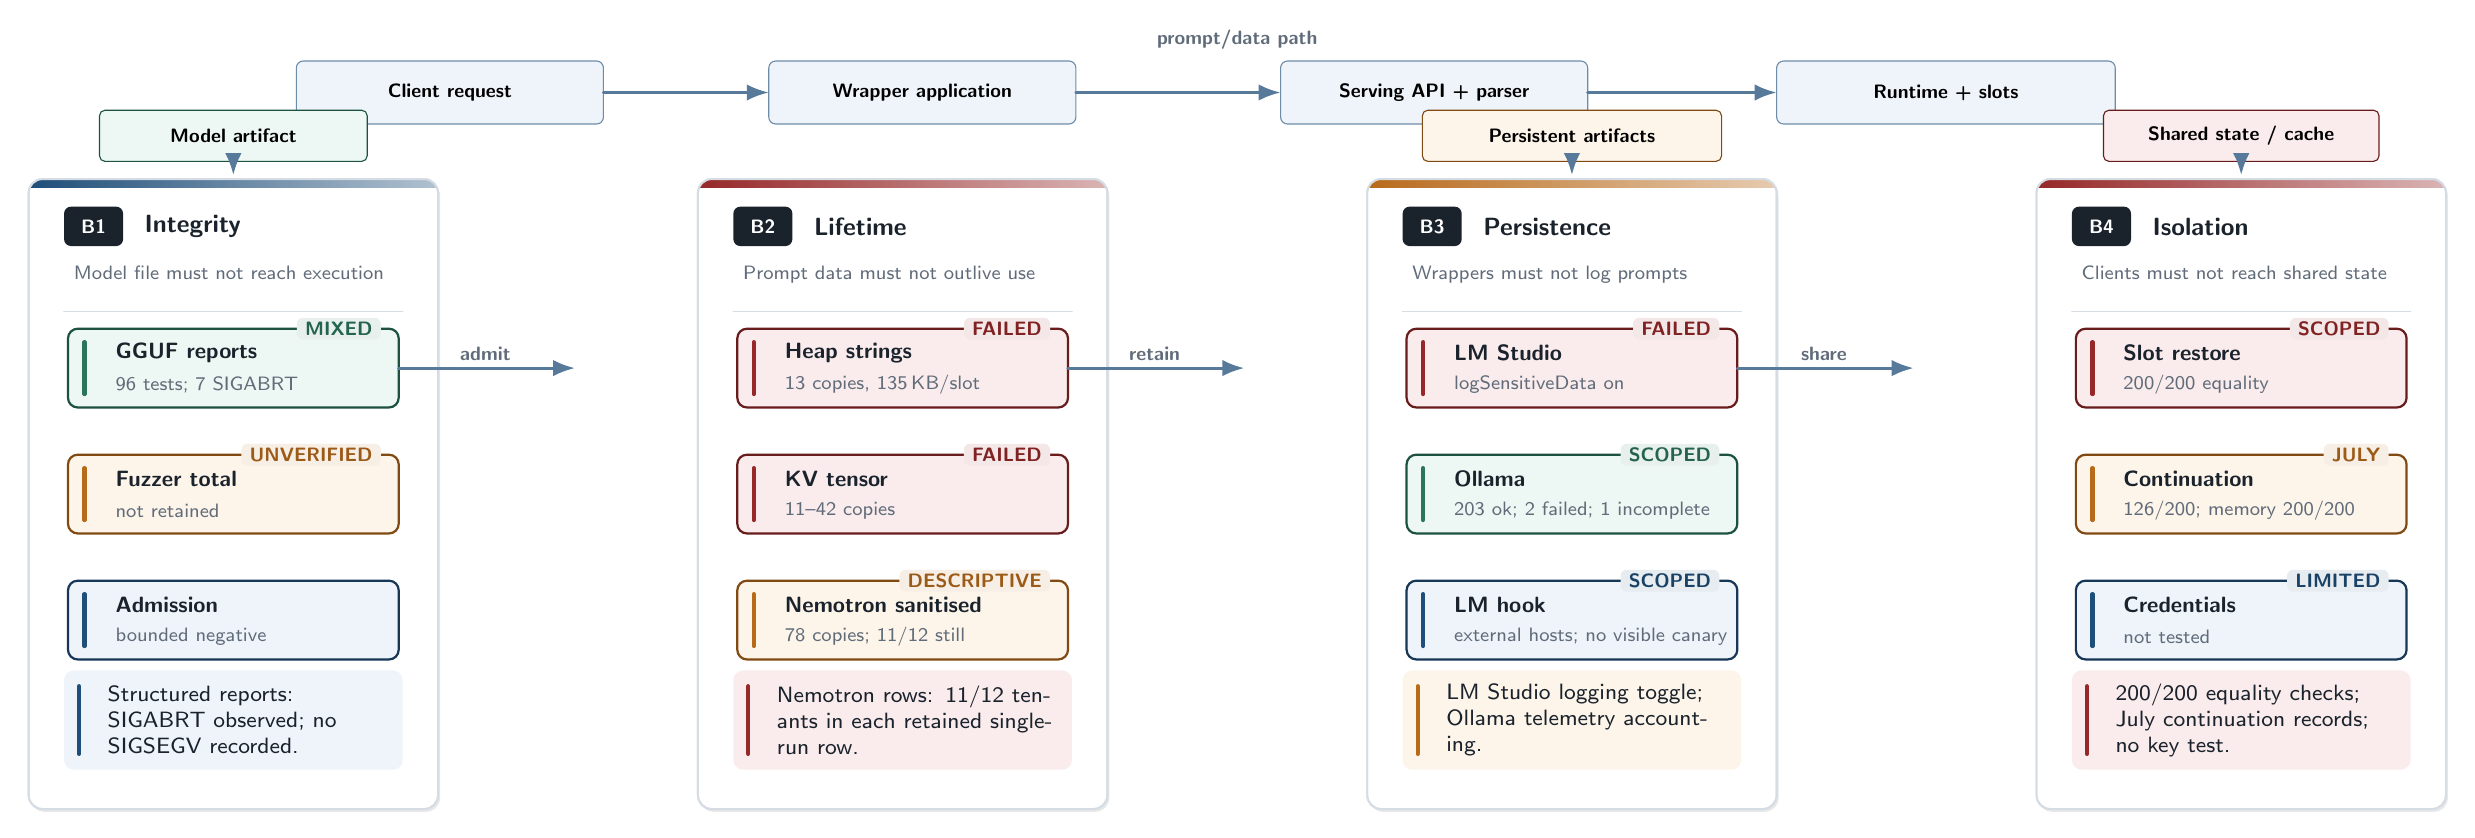
\begin{tikzpicture}[x=1mm,y=1mm,>=Latex,line cap=round,line join=round,font=\sffamily]

		% ================= concrete request/data path =================
		\node[rounded corners=2.5pt, draw=navy!65, fill=navysoft,
		minimum width=39mm, minimum height=8mm, inner sep=1.5pt,
		font=\fsTiny\bfseries] at (-100,51) {Client request};
		\node[rounded corners=2.5pt, draw=navy!65, fill=navysoft,
		minimum width=39mm, minimum height=8mm, inner sep=1.5pt,
		font=\fsTiny\bfseries] at (-40,51) {Wrapper application};
		\node[rounded corners=2.5pt, draw=navy!65, fill=navysoft,
		minimum width=39mm, minimum height=8mm, inner sep=1.5pt,
		font=\fsTiny\bfseries] at (25,51) {Serving API + parser};
		\node[rounded corners=2.5pt, draw=navy!65, fill=navysoft,
		minimum width=43mm, minimum height=8mm, inner sep=1.5pt,
		font=\fsTiny\bfseries] at (90,51) {Runtime + slots};
		\draw[flow] (-80.5,51) -- (-59.5,51);
		\draw[flow] (-20.5,51) -- (5.5,51);
		\draw[flow] (44.5,51) -- (68.5,51);
		\node[elab, anchor=south] at (0,56) {prompt/data path};
		\node[rounded corners=2pt, draw=green!70!black, fill=greensoft,
		minimum width=34mm, minimum height=6.5mm, inner sep=1pt,
		font=\fsTiny\bfseries] at (-127.5,45.5) {Model artifact};
		\draw[flow] (-127.5,42.25) -- (-127.5,40.5);
		\node[rounded corners=2pt, draw=amber!70!black, fill=ambersoft,
		minimum width=38mm, minimum height=6.5mm, inner sep=1pt,
		font=\fsTiny\bfseries] at (42.5,45.5) {Persistent artifacts};
		\draw[flow] (42.5,42.25) -- (42.5,40.5);
		\node[rounded corners=2pt, draw=red!70!black, fill=redsoft,
		minimum width=35mm, minimum height=6.5mm, inner sep=1pt,
		font=\fsTiny\bfseries] at (127.5,45.5) {Shared state / cache};
		\draw[flow] (127.5,42.25) -- (127.5,40.5);

		% ================= B1 Integrity =================
		\begin{scope}[shift={(-127.5,0)}]
			\bchrome{B1}{Integrity}{Model file must not reach execution}{navy}{navysoft}
			{Structured reports: SIGABRT observed; no SIGSEGV recorded.}{26}{52}
			\anode{0}{16}{42}{green}{greensoft}{GGUF reports}{96 tests; 7 SIGABRT}{MIXED}
			\anode{0}{0}{42}{amber}{ambersoft}{Fuzzer total}{not retained}{UNVERIFIED}
			\anode{0}{-16}{42}{navy}{navysoft}{Admission}{bounded negative}{}
		\end{scope}

		% ================= B2 Lifetime =================
		\begin{scope}[shift={(-42.5,0)}]
			\bchrome{B2}{Lifetime}{Prompt data must not outlive use}{red}{redsoft}
			{Nemotron rows: 11/12 tenants in each retained single-run row.}{26}{52}
			\anode{0}{16}{42}{red}{redsoft}{Heap strings}{13 copies, 135\,KB/slot}{FAILED}
			\anode{0}{0}{42}{red}{redsoft}{KV tensor}{11--42 copies}{FAILED}
			\anode{0}{-16}{42}{amber}{ambersoft}{Nemotron sanitised}{78 copies; 11/12 still}{DESCRIPTIVE}
		\end{scope}

		% ================= B3 Persistence =================
		\begin{scope}[shift={(42.5,0)}]
			\bchrome{B3}{Persistence}{Wrappers must not log prompts}{amber}{ambersoft}
			{LM Studio logging toggle; Ollama telemetry accounting.}{26}{52}
			\anode{0}{16}{42}{red}{redsoft}{LM Studio}{logSensitiveData on}{FAILED}
			\anode{0}{0}{42}{green}{greensoft}{Ollama}{203 ok; 2 failed; 1 incomplete}{SCOPED}
			\anode{0}{-16}{42}{navy}{navysoft}{LM hook}{external hosts; no visible canary}{SCOPED}
		\end{scope}

		% ================= B4 Isolation =================
		\begin{scope}[shift={(127.5,0)}]
			\bchrome{B4}{Isolation}{Clients must not reach shared state}{red}{redsoft}
		{200/200 equality checks; July continuation records; no key test.}{26}{52}
			\anode{0}{16}{42}{red}{redsoft}{Slot restore}{200/200 equality}{SCOPED}
			\anode{0}{0}{42}{amber}{ambersoft}{Continuation}{126/200; memory 200/200}{JULY}
			\anode{0}{-16}{42}{navy}{navysoft}{Credentials}{not tested}{LIMITED}
		\end{scope}

		% ================= cross-boundary edges =================
		\draw[flow] (-106.5,16) -- (-84.1,16);
		\draw[flow] (-21.5,16) -- (0.9,16);
		\draw[flow] (63.5,16) -- (85.9,16);
		\node[elab, anchor=south] at (-95.5,16.6) {admit};
		\node[elab, anchor=south] at (-10.5,16.6) {retain};
		\node[elab, anchor=south] at (74.5,16.6) {share};

	\end{tikzpicture}
\end{document}
